% ---------------------------------------------------------------
% Section: Supervised Reference-Calibrated Trajectory Correction
% ---------------------------------------------------------------

\section[Supervised Correction]{Reference-Calibrated Trajectory Correction}

\begin{frame}{Reference-Calibrated Corrector}
\begin{columns}
\begin{column}{0.58\textwidth}
\begin{figure}
    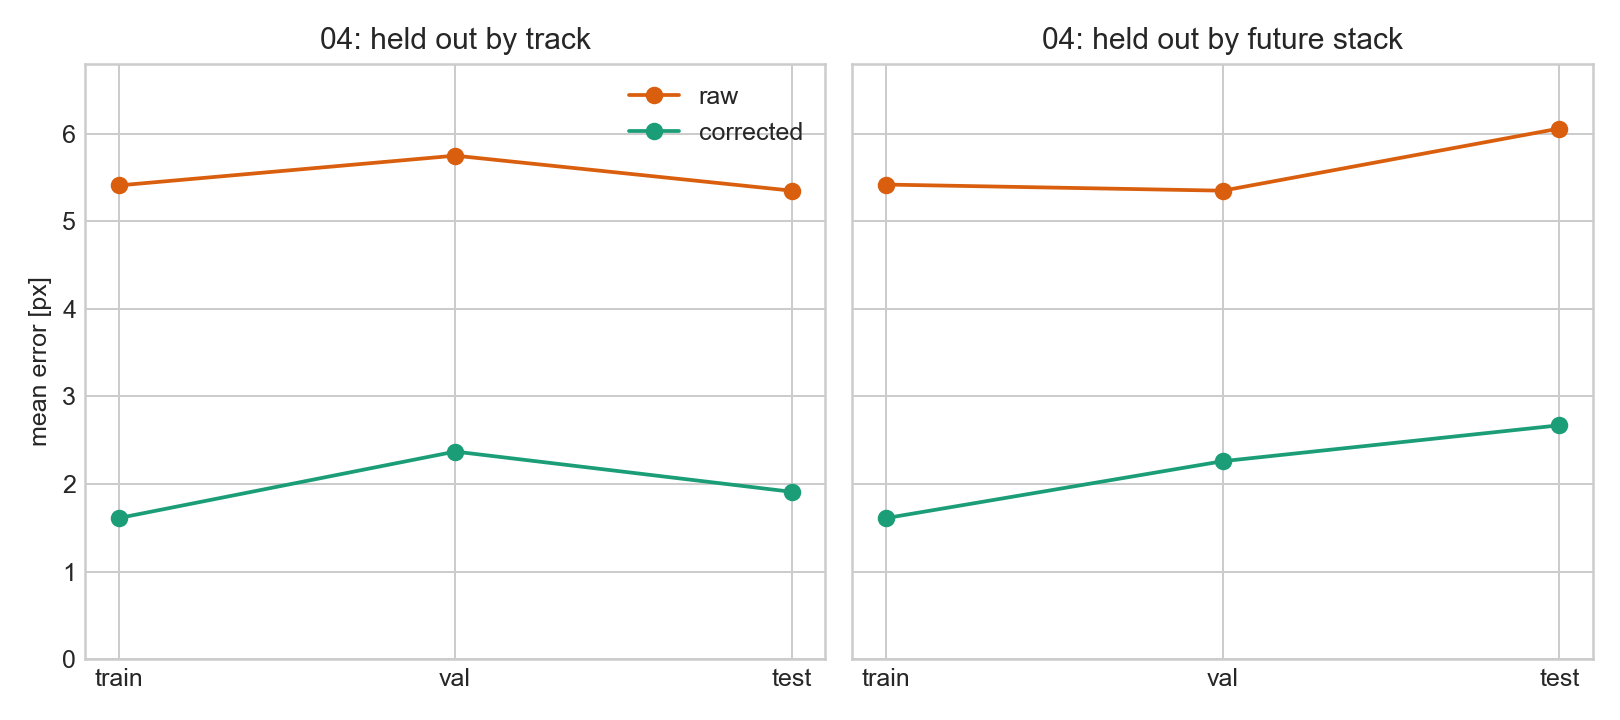
\includegraphics[width=\textwidth]{imglib/progress_update/supervised_correction_error_splits.png}
\end{figure}
\end{column}
\begin{column}{0.42\textwidth}
\begin{myalert}[Framing]
\small The model learns LodeSTAR $\rightarrow$ reference residuals, not ground-truth trajectories.
\end{myalert}
\smallskip
\begin{mynote}
\footnotesize Target: $(x_{\rm ref}-x_{\rm lode}, y_{\rm ref}-y_{\rm lode})$. \\
Leakage feature \texttt{match\_distance} excluded.
\end{mynote}
\end{column}
\end{columns}
\end{frame}

\begin{frame}{Supervised Correction Algorithm}
\begin{columns}
\begin{column}{0.56\textwidth}
\begin{enumerate}\small
    \item Match LodeSTAR detections to reference detections in the same frame
    \item Train on matched pairs only: LodeSTAR features $\rightarrow$ reference residual
    \item Exclude leakage features such as direct match distance
    \item Apply the trained corrector to all LodeSTAR detections
    \item Rebuild/export trajectories from corrected positions
    \item Keep raw, corrected, residual, and quality columns
\end{enumerate}
\end{column}
\begin{column}{0.44\textwidth}
\textbf{Learned target}
\begingroup\footnotesize
\begin{align*}
    r_i &= p^{\rm ref}_i - p^{\rm lode}_i \\
    \hat{r}_i &= f_{\theta}(z^{\rm lode}_i) \\
    p^{\rm corr}_i &= p^{\rm lode}_i + \hat{r}_i
\end{align*}
\endgroup
\begin{mynote}
\footnotesize This is detector calibration, not trajectory hallucination: unmatched LodeSTAR detections can still be corrected after training.
\end{mynote}
\end{column}
\end{columns}
\end{frame}

\begin{frame}{Cross-Dataset Transfer Test}
\begin{columns}
\begin{column}{0.62\textwidth}
\begin{figure}
    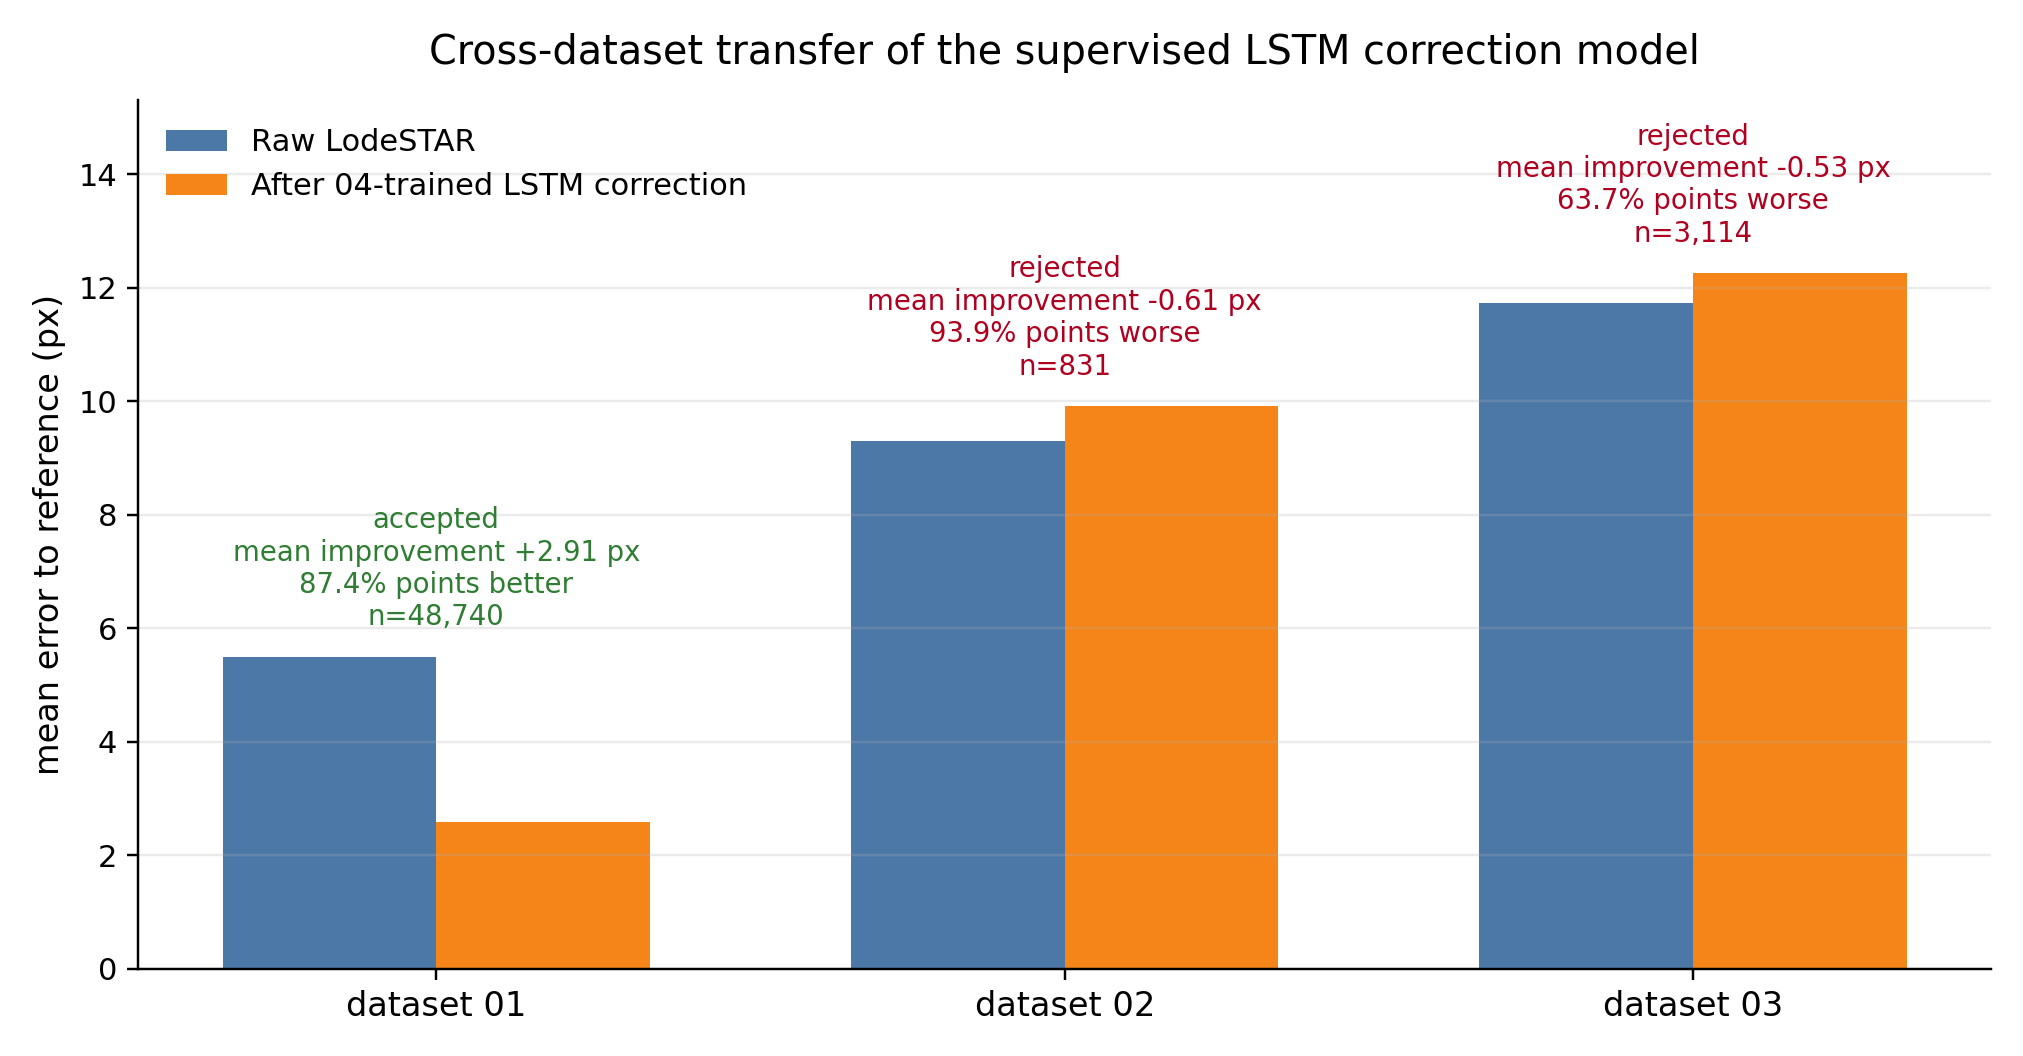
\includegraphics[width=\textwidth]{imglib/progress_update/supervised_transfer_01_02_03_bar.png}
\end{figure}
\end{column}
\begin{column}{0.38\textwidth}
\begin{myalert}[Result]
\small The \texttt{04}-trained corrector transfers to dataset \texttt{01}, but fails on datasets \texttt{02}/\texttt{03}.
\end{myalert}
\smallskip
\begin{mynote}
\footnotesize Transfer is conditional: every new dataset needs a small reference validation gate before accepting corrected trajectories.
\end{mynote}
\end{column}
\end{columns}
\end{frame}

\begin{frame}{Transfer Metrics}
\begin{columns}
\begin{column}{0.54\textwidth}
\begin{table}
\centering
\footnotesize
\begin{tabular}{lrrrr}
\hline
Dataset & Matches & Raw & Corrected & Outcome \\
\hline
\texttt{01} & 48,740 & 5.49 & 2.58 & accepted \\
\texttt{02} & 831 & 9.30 & 9.91 & rejected \\
\texttt{03} & 3,114 & 11.73 & 12.25 & rejected \\
\hline
\end{tabular}
\end{table}
\end{column}
\begin{column}{0.46\textwidth}
\begin{myalert}[Interpretation]
\small The model learned a useful correction for part of the setup family, not a universal LodeSTAR correction.
\end{myalert}
\smallskip
\begin{mynote}
\footnotesize For datasets \texttt{02}/\texttt{03}, keep raw LodeSTAR tracks as the defensible export until a dataset-specific or multi-dataset model is validated.
\end{mynote}
\end{column}
\end{columns}
\end{frame}

\begin{frame}{Dataset \texttt{01}: Refined Trajectories}
\begin{figure}
    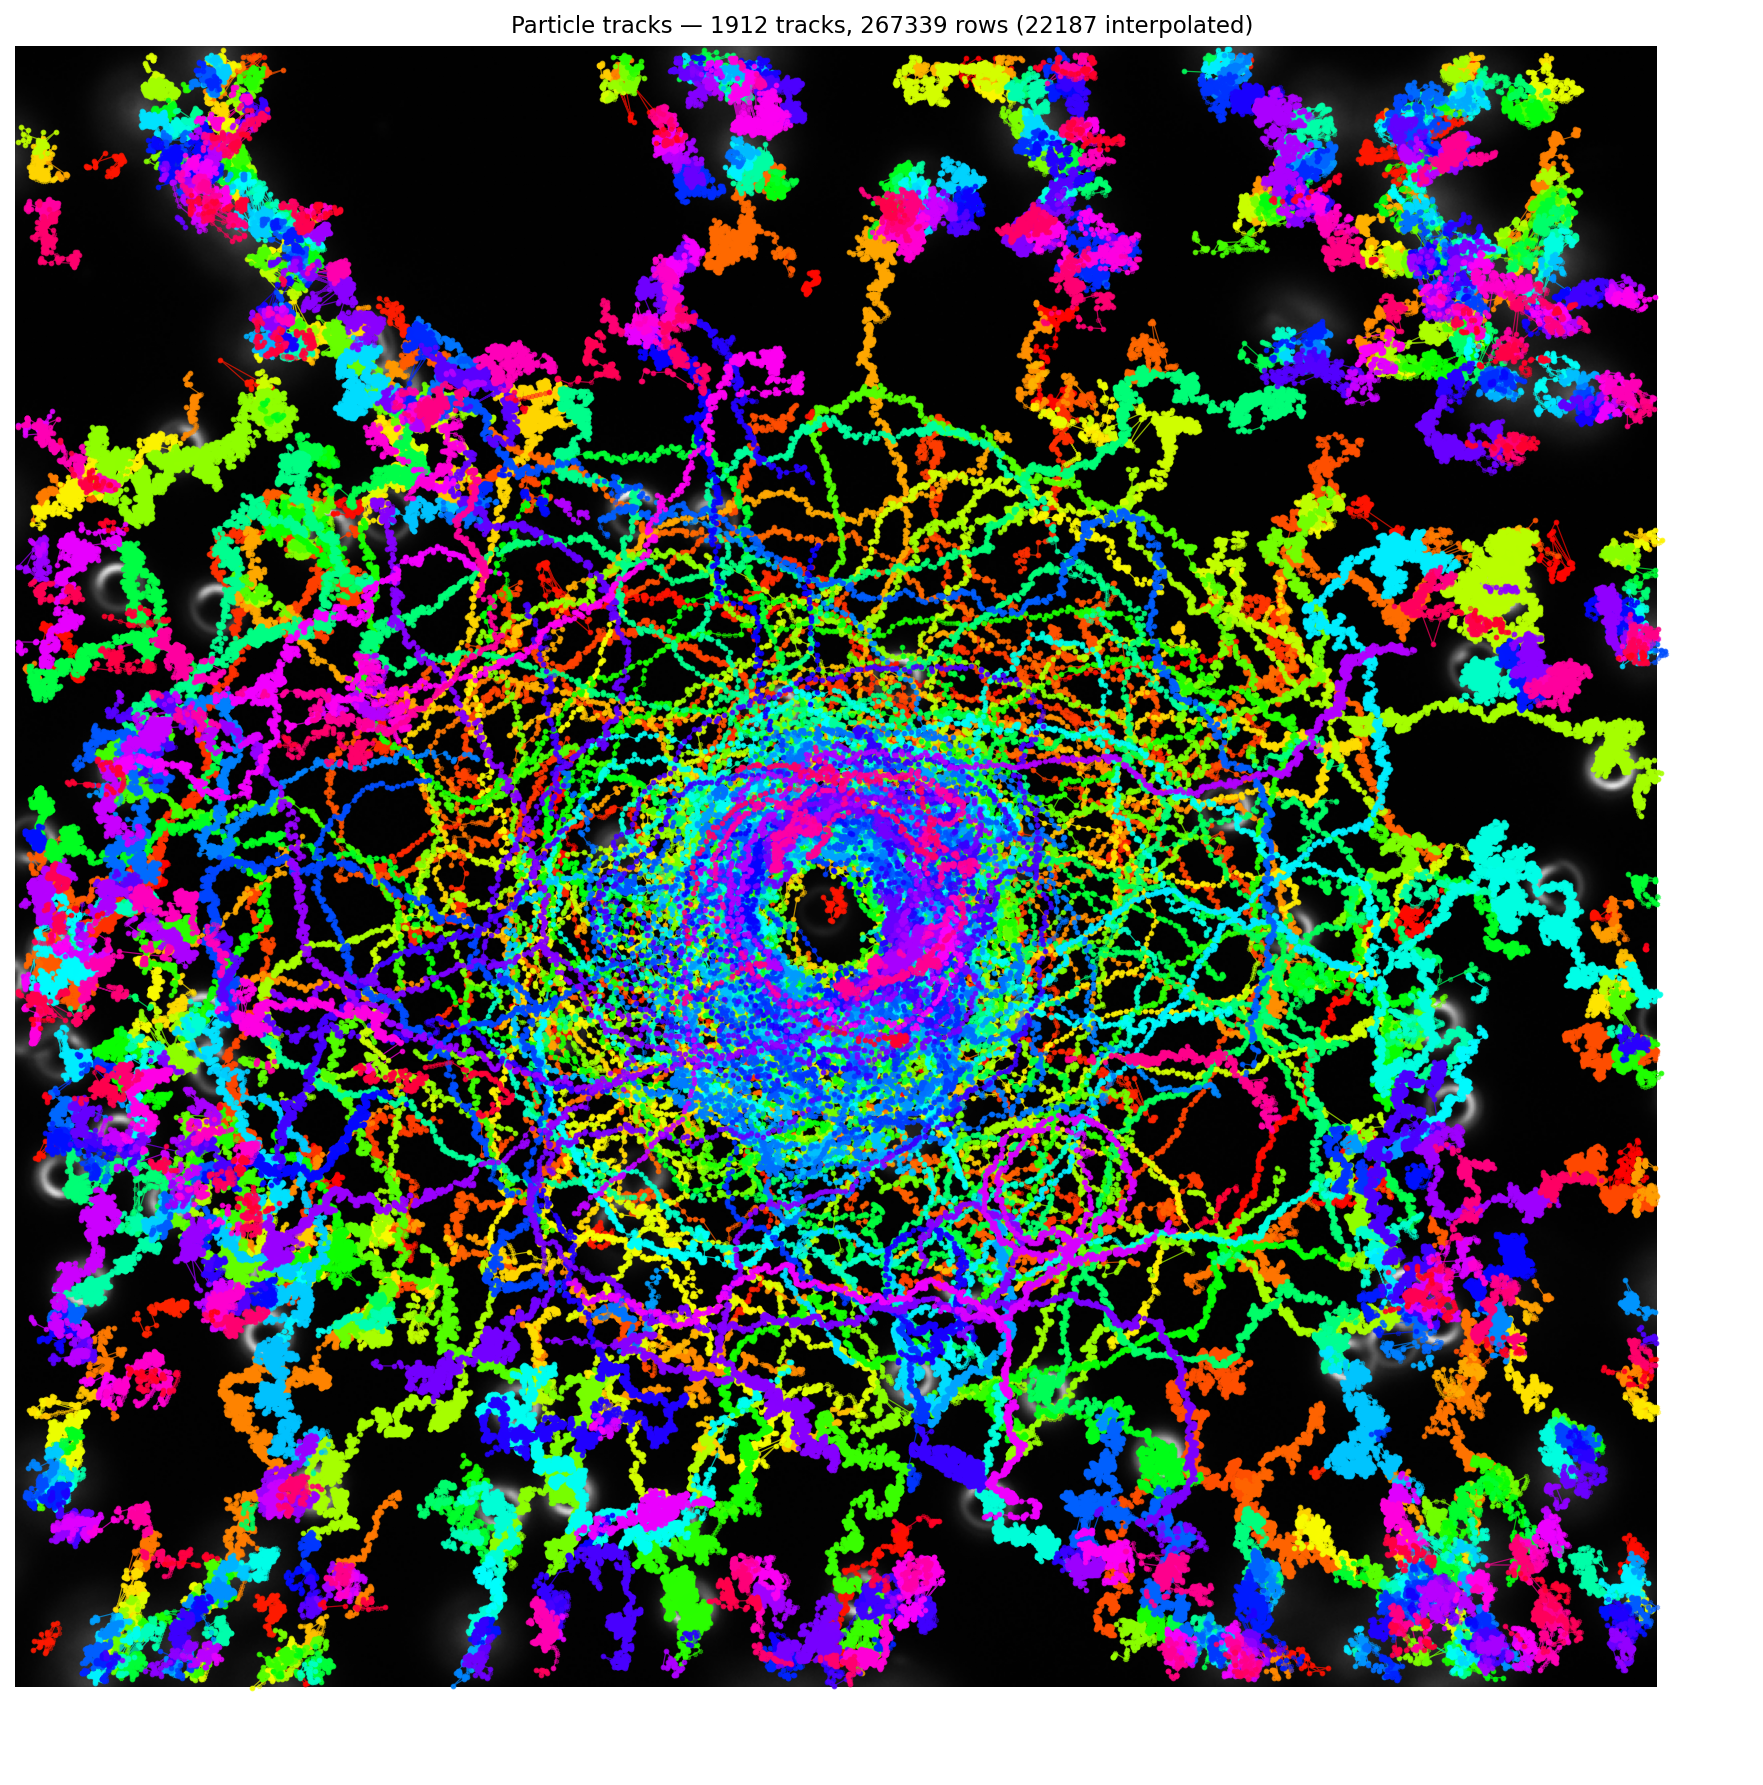
\includegraphics[width=\textwidth, height=0.80\textheight, keepaspectratio]{imglib/progress_update/supervised_refined_overview.png}
\end{figure}
\end{frame}

\begin{frame}{Dataset \texttt{01}: Downstream Checks}
\begin{columns}
\begin{column}{0.5\textwidth}
\begin{figure}
    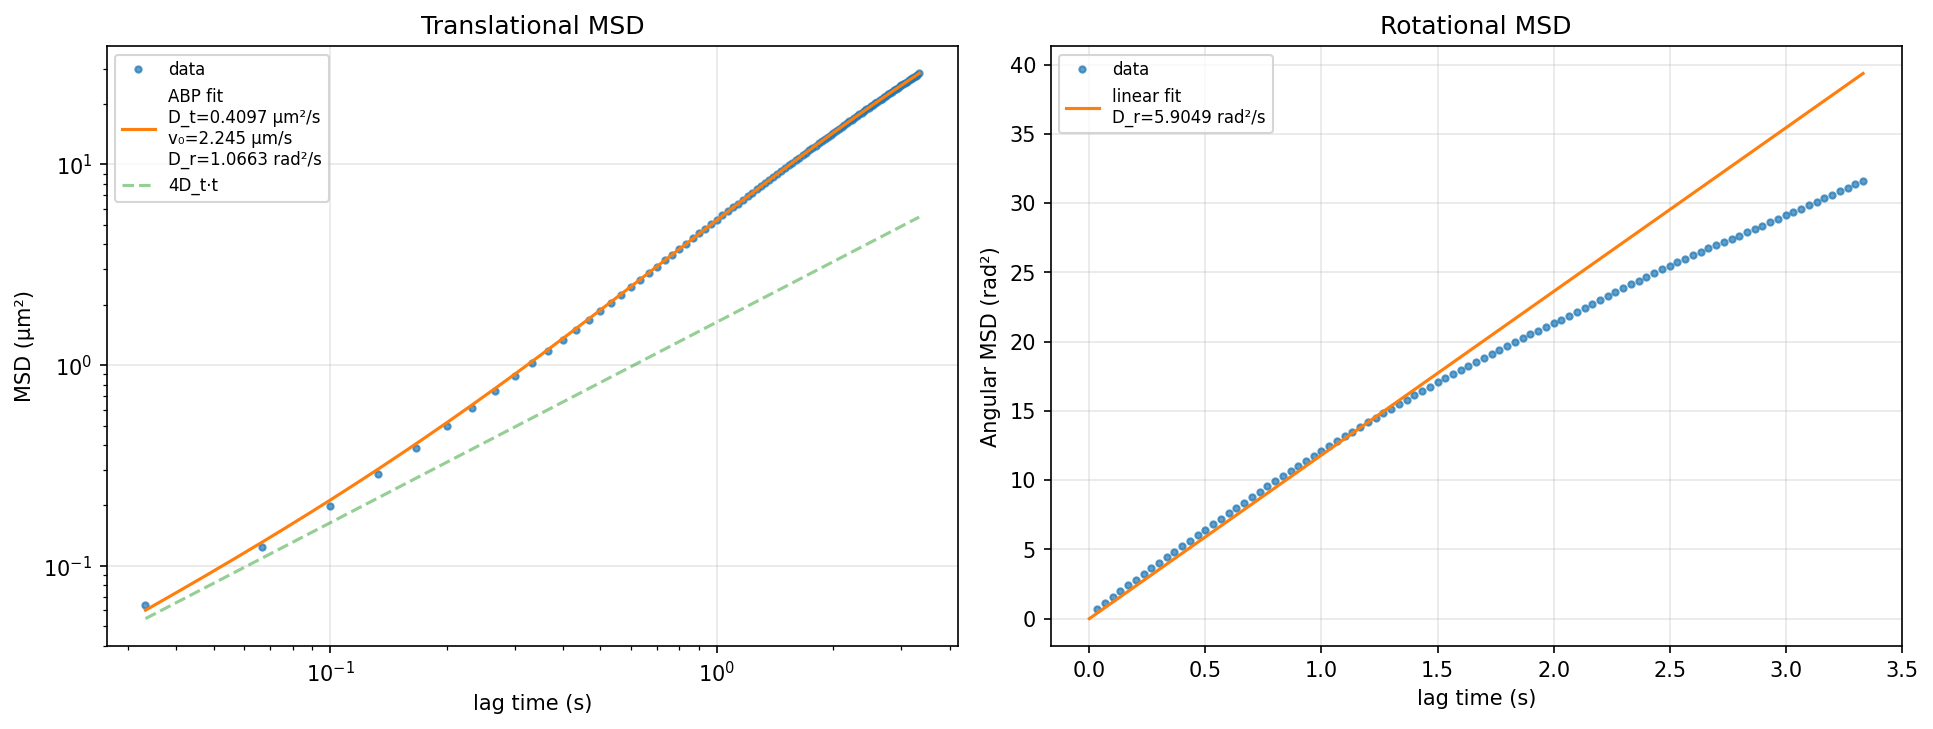
\includegraphics[width=\textwidth, height=0.70\textheight, keepaspectratio]{imglib/progress_update/supervised_refined_msd.png}
\end{figure}
\end{column}
\begin{column}{0.5\textwidth}
\begin{figure}
    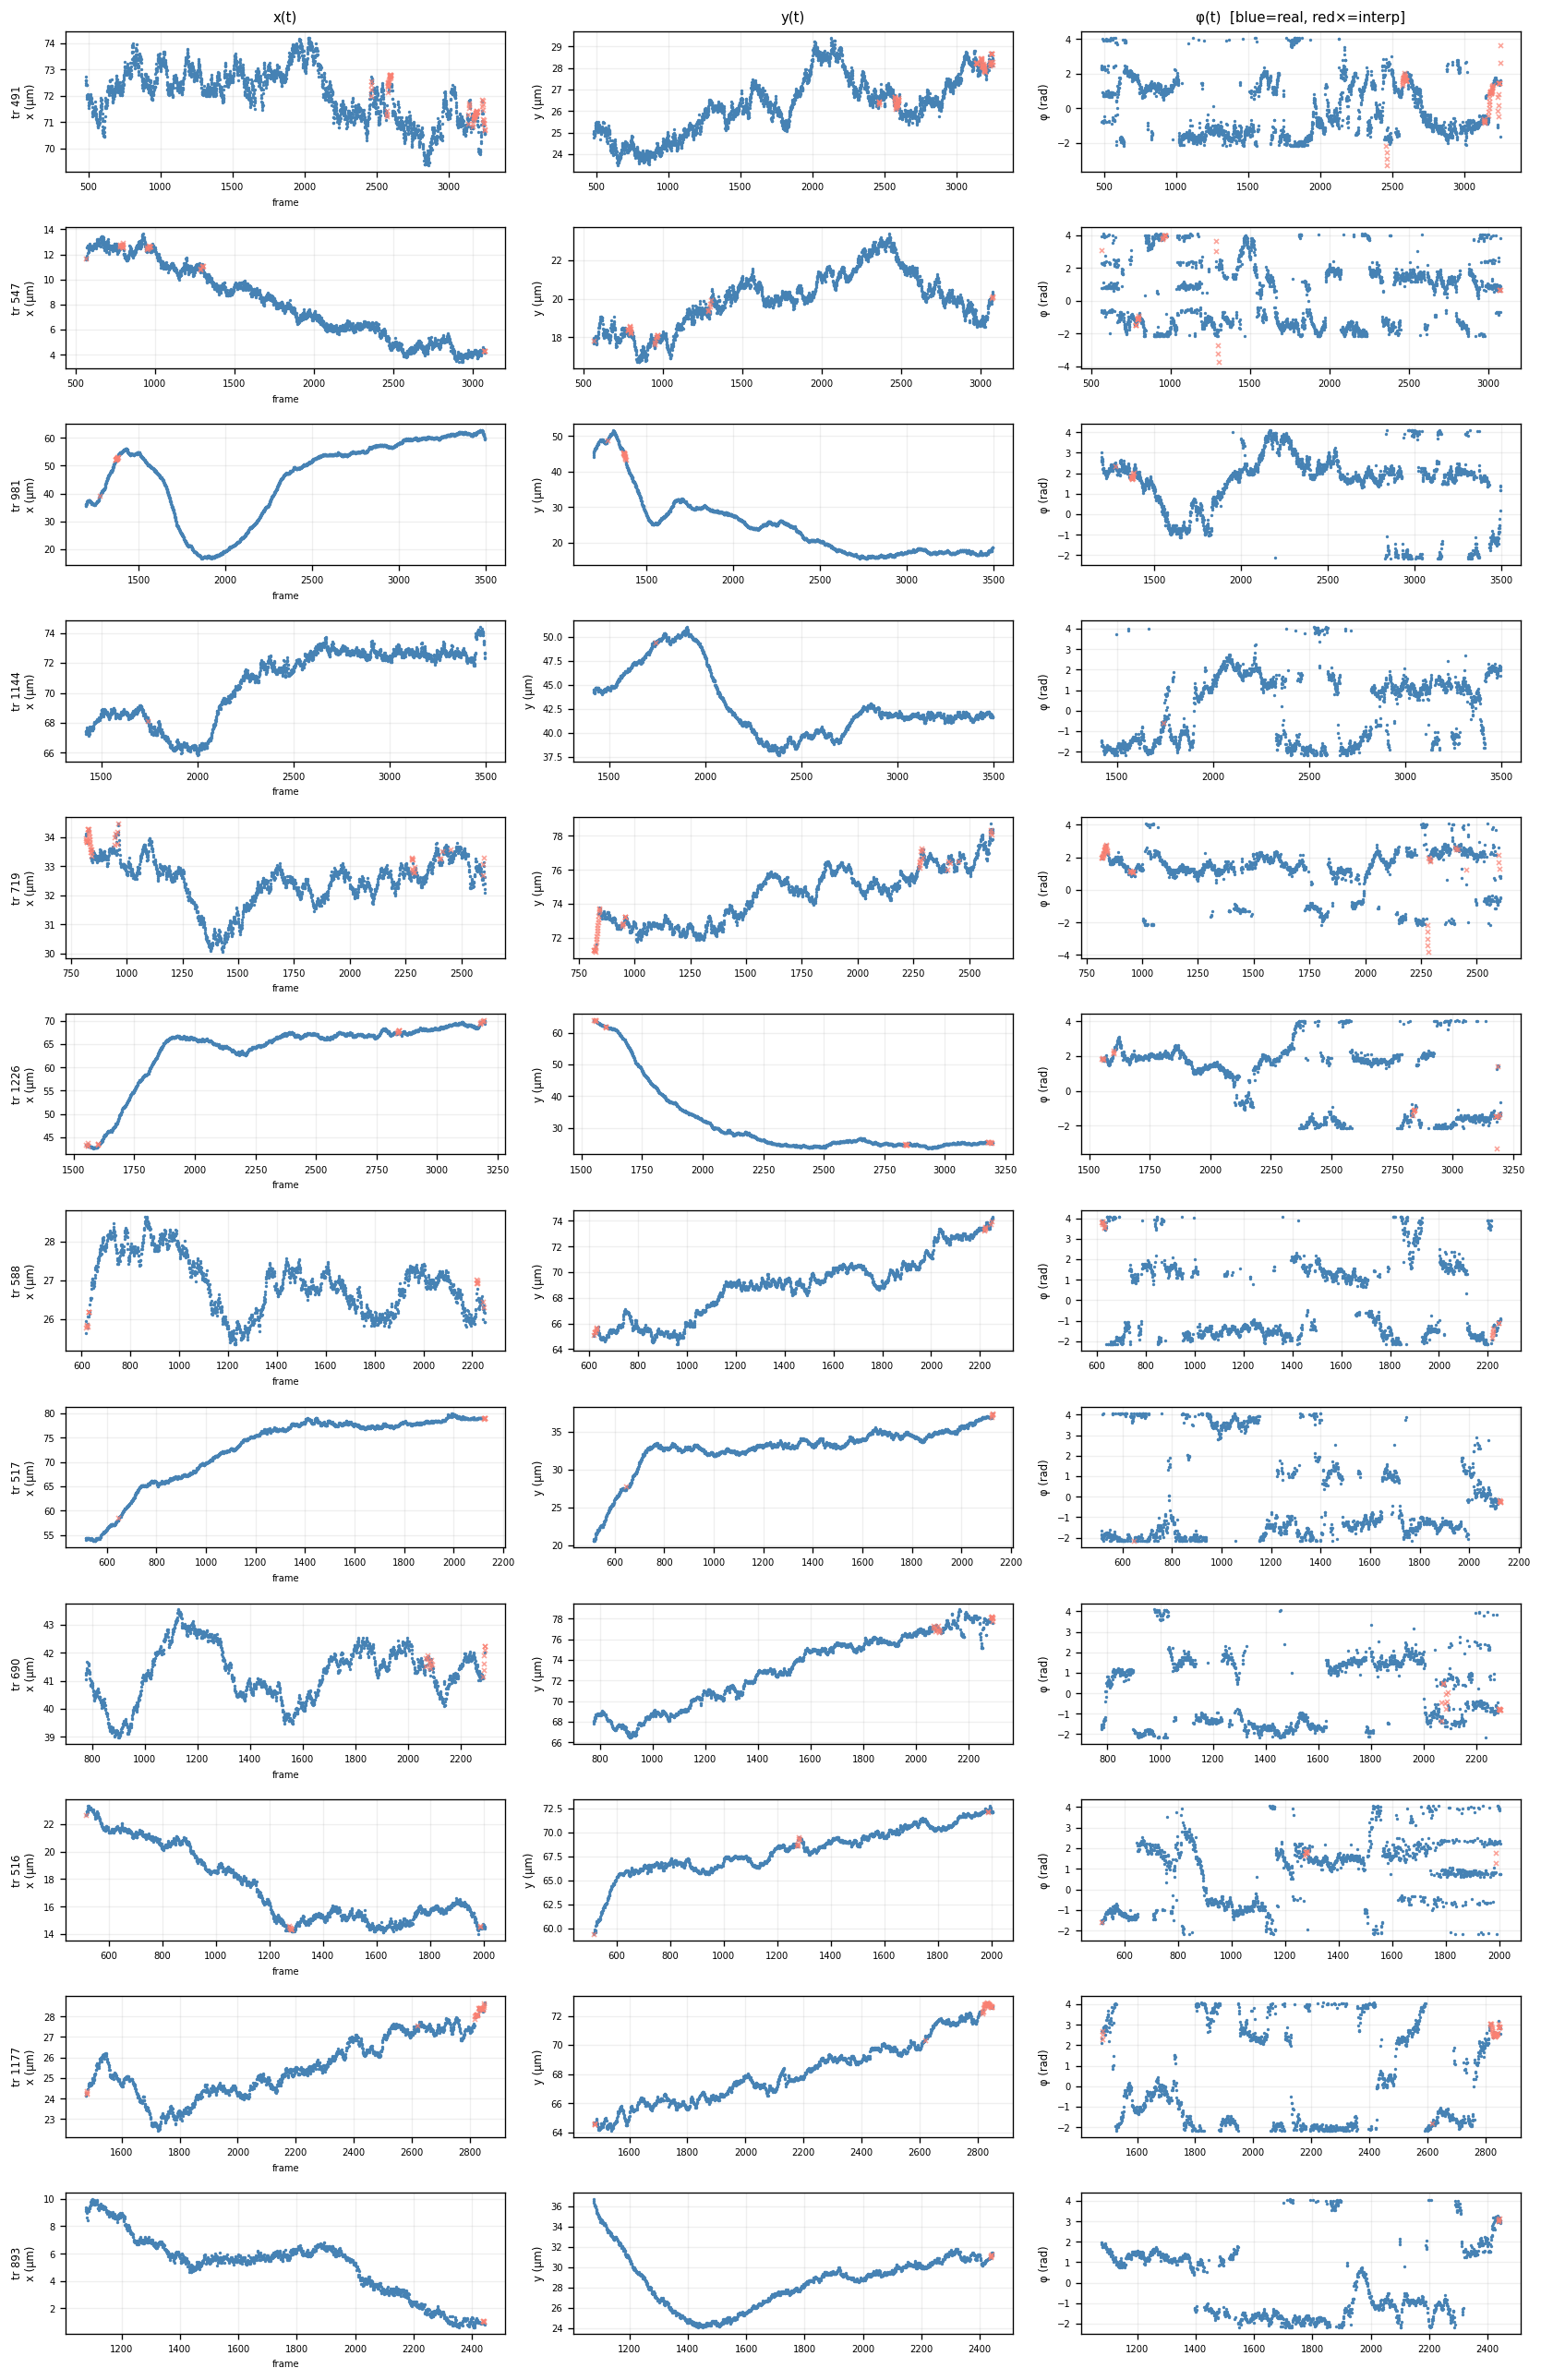
\includegraphics[width=\textwidth, height=0.70\textheight, keepaspectratio]{imglib/progress_update/supervised_refined_sample_tracks.png}
\end{figure}
\end{column}
\end{columns}
\end{frame}
